%!TEX program = xelatex
\documentclass{beamer}

\usepackage{themes/beamerthemeExecushares}
\usepackage{blkarray}
\usepackage{multirow}

\newcommand\sbullet[1][.5]{\mathbin{\vcenter{\hbox{\scalebox{#1}{$\bullet$}}}}}

\newenvironment{rcases}
  {\left.\begin{aligned}}
  {\end{aligned}\right\rbrace}

\title{{Device-Independent}\\{Quantum Key Distribution}\\{(DI-QKD) Secure Against}\\\vspace{0.25ex}{Collective Attacks}}
\subtitle{Non-Locality and Contextuality\\ (2nd Semester - 2023/2024)\\\vspace{-0.75ex} T\'{e}cnico Lisboa, ULisboa}

\author[R.\,A.\,Barreiro]
{%
    \texorpdfstring{
        \begin{columns}
            \column{\linewidth}
            \centering
            {R\'{u}ben Andr\'{e} Barreiro}\\
            \href{mailto:ruben.andre.letra.barreiro@tecnico.ulisboa.pt}{\color{blue}\footnotesize ruben.andre.letra.barreiro@tecnico.ulisboa.pt}
        \end{columns}
    }
    {R\'{u}ben Andr\'{e} Barreiro}
}

\date{\today}

\setcounter{showSlideNumbers}{1}

\begin{document}
	\setcounter{showProgressBar}{0}
	\setcounter{showSlideNumbers}{0}

	\frame{\titlepage}

	\begin{frame}
		\frametitle{Contents}
        
        \vspace{4.5ex}
		\begin{enumerate}
            \item Introduction \\ \textcolor{ExecusharesGrey}{\footnotesize\hspace{1em} - Cryptography in the post-quantum era\\\hspace{1em} - What is a Quantum Key Distribution (QKD) protocol?\\\vspace{-0.75ex}\hspace{1em} - Attacks on QKD protocols}
			\item Problem \\ \textcolor{ExecusharesGrey}{\footnotesize\hspace{1em} - Can a QKD protocol with untrusted quantum devices be secure?}
			\item Motivation \\ \textcolor{ExecusharesGrey}{\footnotesize\hspace{1em} - What is a Device-Independent - Quantum Key Distribution\\\hspace{1.5em} (DI-QKD) protocol?}
			\item Results \\ \textcolor{ExecusharesGrey}{\footnotesize\hspace{1em} - What are the ingredients of a DI-QKD protocol?\\\hspace{1em} - How to prove the security of a DI-QKD protocol?\\\vspace{-0.75ex}\hspace{1em} - Possible loopholes for a DI-QKD protocol}
			\item Conclusions \\ \textcolor{ExecusharesGrey}{\footnotesize\hspace{1em} - Some possible directions and open questions}
		\end{enumerate}
	\end{frame}

	\setcounter{framenumber}{0}
	\setcounter{showProgressBar}{1}
	\setcounter{showSlideNumbers}{1}
    
	\section{Introduction}
 
		\begin{frame}
			\frametitle{\LARGE Cryptography in the post-quantum era}

            \vspace{2ex}
			\begin{itemize}
                \item \textbf{Future quantum threats on cryptography include:}
                \begin{itemize}
                    \item \textbf{Simon's Algorithm}
                    \begin{itemize}
                        \item Brute-force attacks on cryptographic key spaces
                        \item Impact on Advanced Standard Encryption (AES)!
                    \end{itemize}
                    \item \textbf{Grover's Algorithm}
                    \begin{itemize}
                        \item Brute-force attacks on cryptographic key spaces
                        \item AES-128 and AES-192 are no longer secure!
                    \end{itemize}
                    \item \textbf{Brassard-H{\o}yer-Tapp (BHT) Algorithm}
                    \begin{itemize}
                        \item Combination of Grover's algorithm and Birthday Paradox
                        \item SHA-3-224 and SHA-3-256 are no longer secure!
                    \end{itemize}
                    \item \textbf{Shor's Algorithm}
                    \begin{itemize}
                        \item Solves factorization and discrete logarithm problems
                        \item Completely breaks Rivest-Shamir-Adleman (RSA) and Elliptic Curve Cryptography (ECC)!
                    \end{itemize}
                \end{itemize}
                \vspace{1ex}
                \small
                \item \textbf{New public-key cryptography and key exchanges are needed!}
            \end{itemize}
		\end{frame}

    \begin{frame}
        \frametitle{\LARGE Cryptography in the post-quantum era}
        
        \vspace{2.5ex}
        \begin{itemize}
            \item \textbf{Two new main approaches arise...}
            \begin{table}[]
                \centering
                \resizebox{0.9\columnwidth}{!}{%
                    \begin{tabular}{|c|c|c|}
                        \hline
                        \multirow{2}{*}{\textbf{}} &
                        \textbf{(Classical)} &
                        \multirow{2}{*}{\textbf{Quantum Cryptography}} \\
                        &
                        \textbf{Post-Quantum Cryptography} &
                        \\ \hline
                        \textbf{Foundation} &
                        \begin{tabular}[c]{@{}c@{}}(Still Believed) Hard\\ Mathematical Problems\end{tabular} &
                        Quantum Mechanics and Physics \\ \hline
                        \textbf{Type of Information} &
                        Classical &
                        (Mainly) Quantum \\ \hline
                        \textbf{Encoding} &
                        N/A &
                        \begin{tabular}[c]{@{}c@{}}Discrete-Variables (DV) for qubits\\ or Continuous-Variables (CV) for qumodes\end{tabular} \\ \hline
                        \textbf{Strategies} &
                        N/A &
                        Prepare-and-Measure or Entanglement \\ \hline
                        \textbf{Families} &
                        \begin{tabular}[c]{@{}c@{}}Lattice-based, Code-based,\\ Hash-based, Isogeny-based,\\ Multivariate, and\\ Zero-Knowledge Proofs (ZKPs)\end{tabular} &
                        \begin{tabular}[c]{@{}c@{}}Quantum Key Distribution (QKD),\\ Semi-Quantum Key Distribution (QKD),\\ Quantum Conference Key Agreement (QCKA),\\ Quantum Digital Signature Scheme (QDSS),\\ Quantum Bit Commitment (QBC),\\ Quantum Oblivious Transfer (QOT),\\ and Quantum Multi-Party Computation (QMPC)\end{tabular} \\ \hline
                        \textbf{Popular Primitives} &
                        \begin{tabular}[c]{@{}c@{}}CRYSTALS-Kyber,\\ CRYSTALS-Dilithium,\\ FALCON, SPHINCS+, McEliece,\\ HQC, and BIKE\end{tabular} &
                        \begin{tabular}[c]{@{}c@{}}BB84, B92, SSP, SARG04,\\ E91, BBM92, KMB09, T12,\\ Decoy State, Squeezed State,\\ DPS, MSZ96, GG02\end{tabular} \\ \hline
                    \end{tabular}%
                }
                \caption{\color{blue}{Table 1: }\color{black}Overview of the two main approaches for cryptography in the post-quantum era}
                \label{tab:overview-main-approaches-cryptography-post-quantum-era}
            \end{table}
        \end{itemize}
    \end{frame}

		\begin{frame}
			\frametitle{\large What is a Quantum Key Distribution (QKD) protocol?}

            \vspace{4ex}
            \begin{figure}
                \centering
                \begin{minipage}{0.5\textwidth}
                    \centering
                    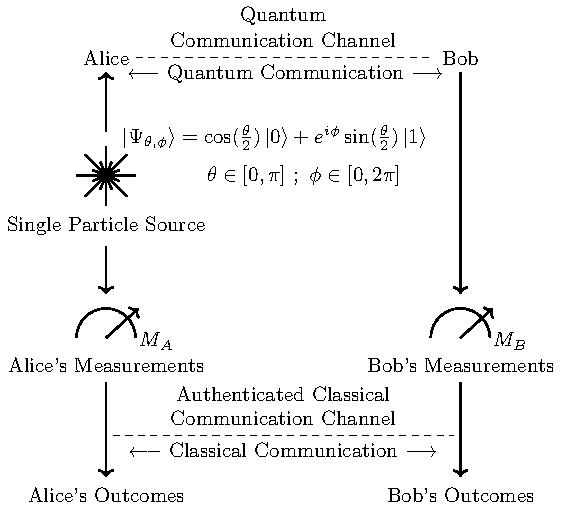
\includegraphics[width=0.95\linewidth, height=0.5\textheight]{figures/presentation/pdf/prepare-and-measure-qkd-protocol.pdf}
                    \vspace{-1.5ex}
                    \caption{\color{blue}{Figure 1a: }\color{black}{\tabular[t]{@{}l@{}}High-level procedure schematic of\\ a Prepare-and-Measure QKD protocol\endtabular}}
                    \label{fig:prepare-measure-qkd-protocol}
                \end{minipage}%
                \begin{minipage}{0.5\textwidth}
                    \centering
                    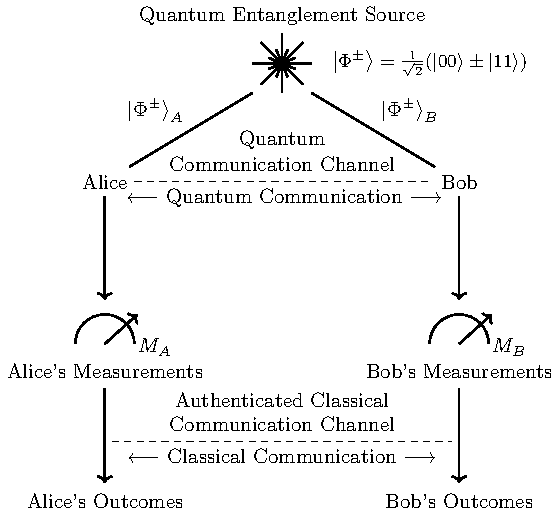
\includegraphics[width=0.95\linewidth, height=0.5\textheight]{figures/presentation/pdf/entanglement-based-qkd-protocol.pdf}
                    \vspace{-1.5ex}
                    \caption{\color{blue}{Figure 1b: }\color{black}{\tabular[t]{@{}l@{}}High-level procedure schematic of\\ an Entanglement-based QKD protocol\endtabular}}
                    \label{fig:entanglement-based-qkd-protocol}
                \end{minipage}
            \end{figure}
   
		\end{frame}

		\begin{frame}
			\frametitle{\large What is a Quantum Key Distribution (QKD) protocol?}

            \vspace{4ex}
            \begin{figure}
                \centering
                \begin{minipage}{0.4\textwidth}
                    \centering
                    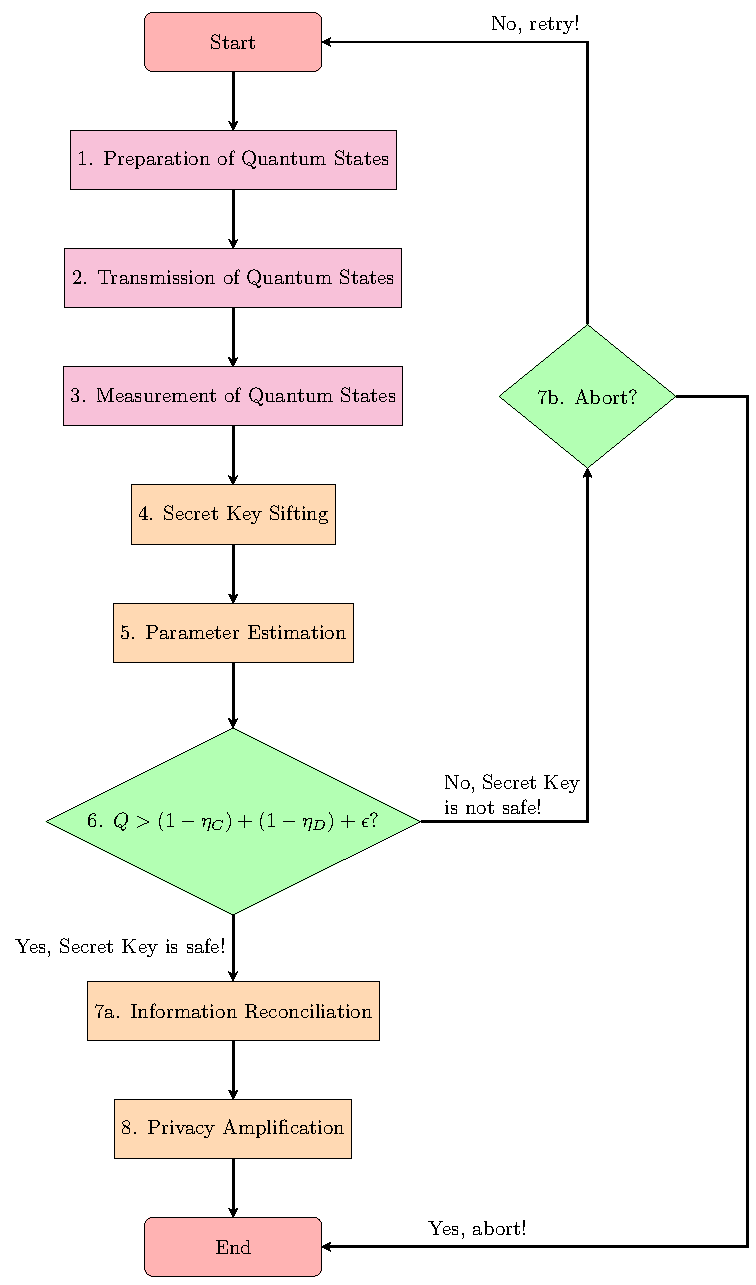
\includegraphics[width=1.0\linewidth, height=0.75\textheight]{figures/presentation/pdf/qkd-protocol-flowchart.pdf}
                    \vspace{-4ex}
                    \caption{\color{blue}{Figure 2: }\color{black}{Flowchart of a QKD protocol}}
                    \label{fig:qkd-protocol-flowchart-1}
                \end{minipage}%
                \hspace{0.05\textwidth}%
                \begin{minipage}{0.55\textwidth}
                    \begin{enumerate}\footnotesize
                        \item \textbf{Preparation of Quantum States}
                        \begin{itemize}\scriptsize
                            \item Single Particles, Entangled Particles, Coherent States, Fock States, etc.
                        \end{itemize}
                        \item \textbf{Transmission of Quantum States}
                        \begin{itemize}\scriptsize
                            \item Uses a quantum communication channel with a certain efficiency ${\eta}_{C}$
                            \item ``Flying'' quantum states can be eavesdropped, introducing a noise $\epsilon$
                        \end{itemize}
                        \item \textbf{Measurement of Quantum States}
                        \begin{itemize}\scriptsize
                            \item Uses quantum measurement devices with a certain efficiency ${\eta}_{D}$
                            \item Composes a raw key
                        \end{itemize}
                        \item \textbf{Secret Key Sifting}
                        \begin{itemize}\scriptsize
                            \item Identifies which protocol rounds can be used to compose a sifted key
                        \end{itemize}
                    \end{enumerate}
                \end{minipage}
            \end{figure}
   
		\end{frame}
  

		\begin{frame}
			\frametitle{\large What is a Quantum Key Distribution (QKD) protocol?}

            \vspace{4ex}
            \begin{figure}
                \centering
                \begin{minipage}{0.4\textwidth}
                    \centering
                    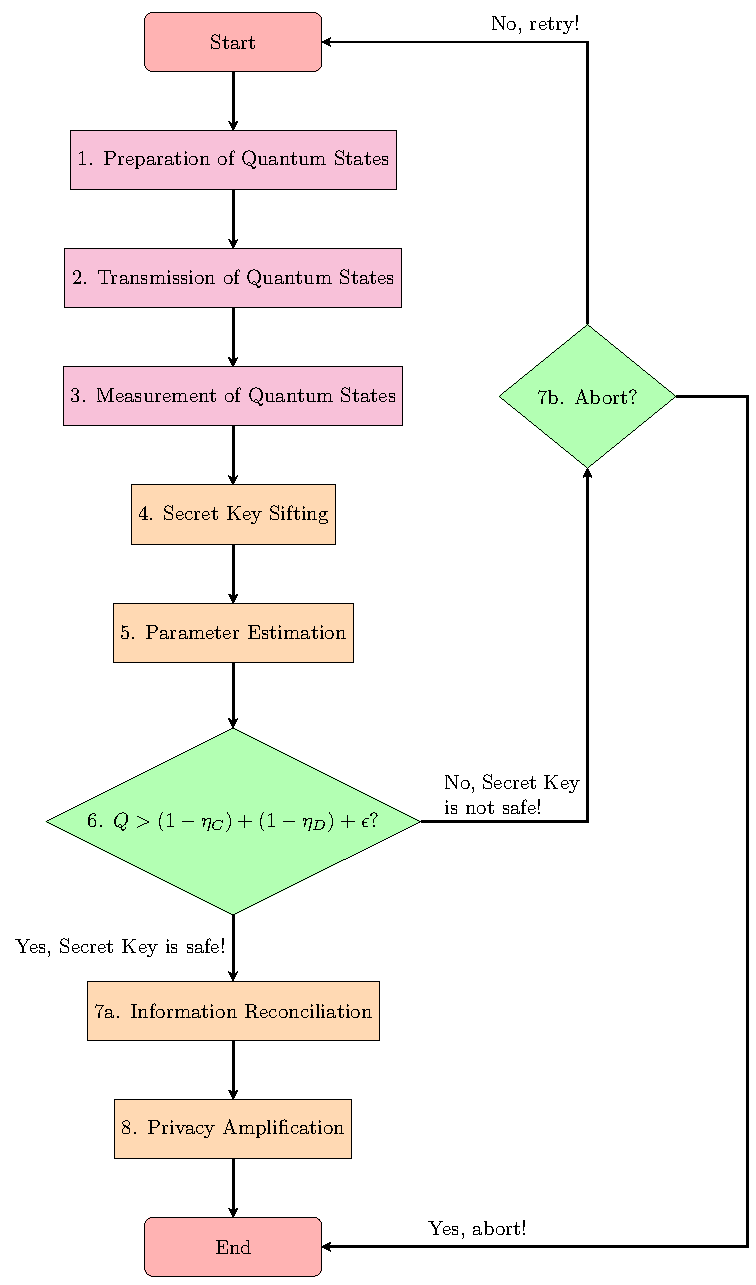
\includegraphics[width=1.0\linewidth, height=0.75\textheight]{figures/presentation/pdf/qkd-protocol-flowchart.pdf}
                    \vspace{-4ex}
                    \caption{\color{blue}{Figure 2: }\color{black}{Flowchart of a QKD protocol}}
                    \label{fig:qkd-protocol-flowchart-2}
                \end{minipage}%
                \hspace{0.05\textwidth}%
                \begin{minipage}{0.55\textwidth}
                    \begin{enumerate}\footnotesize
                        \item[5.] \textbf{Parameter Estimation}
                        \begin{itemize}\scriptsize
                            \item Samples and evaluates\\ the Quantum Bit Error Rate (QBER) $Q$
                            \item Estimates the key rate
                            \item Estimates the secure mutual information between Alice and Bob
                            \item Estimates the Holevo bound
                        \end{itemize}
                        \item[6.] (\textbf{Eavesdropping detected?})\\$\Rightarrow$ $Q > (1 - {\eta}_{C}) + (1 - {\eta}_{D}) + \epsilon$\ ?
                        \begin{enumerate}\scriptsize
                            \item[7a.] Yes! $\Rightarrow$ \textbf{Information Reconciliation}
                            \begin{itemize}\scriptsize
                                \item Applies an Error Correction Code (ECC) to correct the sifted into an error-free key
                                \item These ECC algorithms include:\\
                                - \textbf{Cascade protocol, Winnow\\\hspace{1ex}protocol, and Low-Density\\\hspace{1ex}Parity-Check (LDPC) codes}
                                \item Can be accelerated by classical software and hardware\\(e.g., \textbf{OpenMP}, \textbf{CUDA}, etc.)
                            \end{itemize}
                            \item[7b.] No! $\Rightarrow$ Abort? (or Retry?)
                        \end{enumerate}
                    \end{enumerate}
                \end{minipage}
            \end{figure}
   
		\end{frame}
  

		\begin{frame}
			\frametitle{\large What is a Quantum Key Distribution (QKD) protocol?}

            \vspace{4ex}
            \begin{figure}
                \centering
                \begin{minipage}{0.4\textwidth}
                    \centering
                    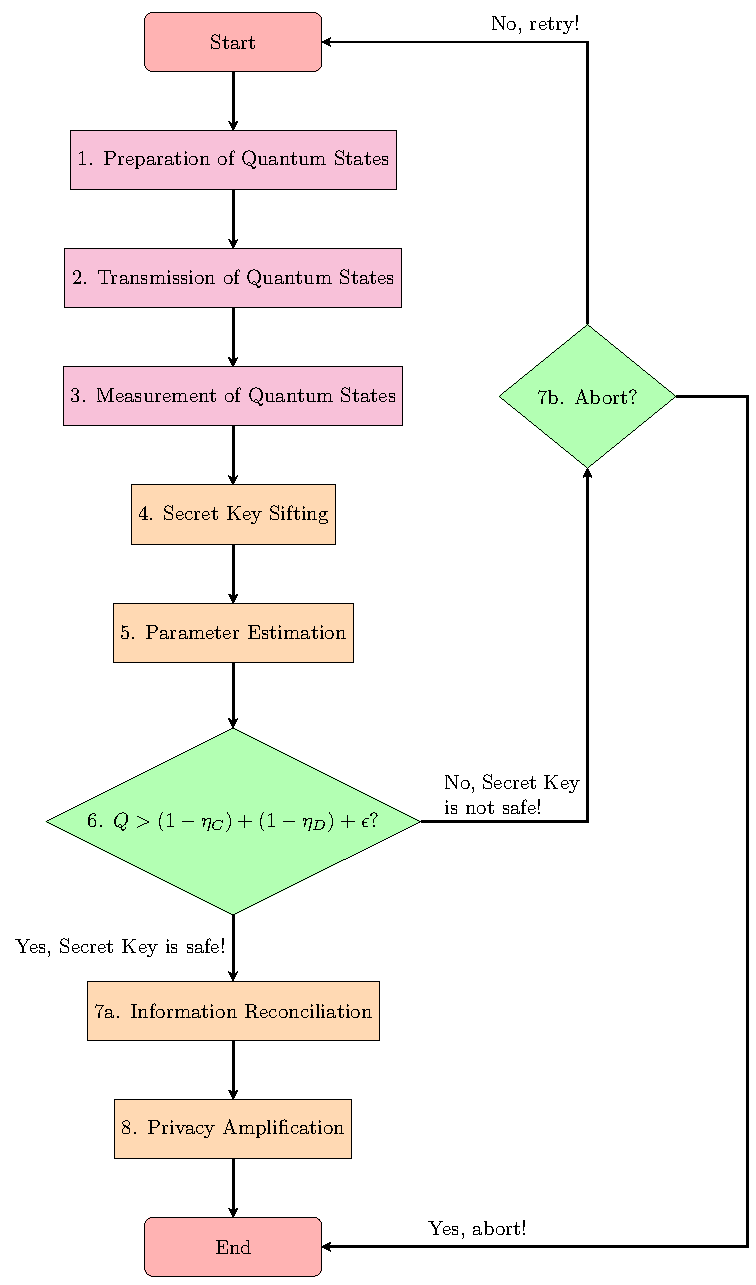
\includegraphics[width=1.0\linewidth, height=0.75\textheight]{figures/presentation/pdf/qkd-protocol-flowchart.pdf}
                    \vspace{-4ex}
                    \caption{\color{blue}{Figure 2: }\color{black}{Flowchart of a QKD protocol}}
                    \label{fig:qkd-protocol-flowchart-3}
                \end{minipage}%
                \hspace{0.05\textwidth}%
                \begin{minipage}{0.55\textwidth}
                    \begin{enumerate}\footnotesize
                        \item[8.] \textbf{Privacy Amplification Estimation}
                        \begin{itemize}\scriptsize
                            \item Applies a Universal Hash Function on the error-free key, composing the final (and amplified) secret key
                            \item This Universal Hash Function can be a \textbf{Toeplitz Hashing} procedure, usually applied using a random seed as well
                            \item Can be accelerated by classical software and hardware\\(e.g., \textbf{OpenMP}, \textbf{CUDA}, etc.)
                        \end{itemize}
                    \end{enumerate}

                    \begin{itemize}\scriptsize
                        \item The \textbf{Secret Key Sifting}, \textbf{Parameter\\ Estimation}, \textbf{Information Reconciliation},\\ and \textbf{Privacy Amplification} steps require\\ an authenticated and interactive exchange\\ of classical information/messages\\
                        \begin{itemize}\scriptsize
                            \item We can achieve it with\\ a \textbf{Carter-Wegman Message Authentication Code (CW-MAC)}, requiring an initial small secret defined \textit{a priori}
                        \end{itemize}
                    \end{itemize}
                \end{minipage}
            \end{figure}
   
		\end{frame}
  

		\begin{frame}
			\frametitle{\Large Attacks on QKD protocols}

            \vspace{4ex}
            \begin{itemize}
                \item \textbf{\textit{Independent and identically distributed} (\textit{i.i.d.}) rounds:}
                \vspace{-2.5ex}
                \begin{itemize}
                    \item The devices behave independently and in the same way
                    \item The quantum states distributed are always the same
                \end{itemize}
                \vspace{0.5ex}
                \item \textbf{There are three main attacks on QKD protocols:}
                \begin{itemize}
                    \item \textbf{Individual Attacks:}
                    \begin{itemize}
                        \footnotesize
                        \item The eavesdropper has no quantum memory\\
                        \footnotesize
                        \item The eavesdropper can only attack individually each round
                    \end{itemize}
                    \item \textbf{Collective Attacks:}
                    \begin{itemize}
                        \footnotesize
                        \item The eavesdropper has no quantum memory\\
                        \footnotesize
                        \item The eavesdropper can perform arbitrary global operations
                    \end{itemize}
                    \item \textbf{Coherent Attacks:}
                    \begin{itemize}
                        \footnotesize
                        \item The eavesdropper has quantum memory (trace of rounds)\\
                        \footnotesize
                        \item The eavesdropper can perform arbitrary global operations\\
                        \footnotesize
                        \item The parties' quantum states can be arbitrarily correlated
                    \end{itemize}
                \end{itemize}
            \end{itemize}
   
		\end{frame}

  
	\section{Problem}

		\begin{frame}
			\frametitle{\normalsize Can a QKD protocol with untrusted quantum devices be secure?}

            \vspace{2.5ex}
            \begin{itemize}
                \item \textbf{Considering Entanglement-based QKD protocols:}
                \begin{itemize}\small
                    \item The entangled particles are emitted from a common source
                    \item The parties measure each particle on a randomly chosen basis
                    \vspace{0.5ex}
                    \item Here, we assume that:
                    \begin{itemize}
                        \item The locations of the parties (Alice and Bob) are secure
                        \item Alice and Bob trust their measuring devices
                    \end{itemize}
                    \vspace{0.5ex}
                    \item The source of the entangled particles:
                    \begin{itemize}
                        \item Does not need to be trusted by Alice and Bob
                        \item Might be under the control of an eavesdropper (Eve)
                    \end{itemize}
                \end{itemize}
                \vspace{1ex}
                \item \textbf{And about untrusted quantum measurement devices?}
                \vspace{-2.5ex}
                \begin{itemize}
                    \item No guarantees on the expected measurement bases
                    \item No assumptions on the dimension of the Hilbert Space
                \end{itemize}
            \end{itemize}
		\end{frame}

    \section{Motivation}

		\begin{frame}
			\frametitle{\footnotesize What is a Device‑Independent ‑ Quantum Key Distribution (DI‑QKD) protocol?}

            \vspace{2.5ex}
            \begin{itemize}
                \item \textbf{Device‑Independent ‑ Quantum Key Distribution (DI‑QKD)} is a concept of security for QKD protocols that:
                \begin{itemize}
                    \item \textbf{Seeks to ensure the security of QKD protocols:}
                    \begin{itemize}
                        \item \textbf{Without considering any details about the internal working of the quantum devices being used:}\\
                        - The quantum devices can be imperfect,\\\hspace{0.5em}untrusted, or manipulated by a malicious party
                        \item \textbf{Based on the violation of Bell Inequalities}, ensuring:\\
                        - Quantum correlations between the quantum devices\\
                        - The security is inferred directly from those\\\hspace{0.5em}quantum correlations observed on the outcomes\\
                        - Do not exist any local hidden variables
                    \end{itemize}
                    \vspace{0.5ex}
                    \item \textbf{It is a ``holy-grail'' on Quantum Cryptography!}
                \end{itemize}
            \end{itemize}
		\end{frame}

		\begin{frame}
			\frametitle{\footnotesize What is a Device‑Independent ‑ Quantum Key Distribution (DI‑QKD) protocol?}

            \vspace{2.5ex}
            \begin{itemize}
                \item \textbf{Device‑Independent ‑ Quantum Key Distribution (DI‑QKD)} requires the following basic assumptions:
                \begin{itemize}
                    \normalsize
                    \item \textbf{The physical locations of the parties are secure}\\
                    \small
                    - No unwanted information can leak out to the outside
                    \normalsize
                    \item \textbf{The parties have a Trusted Random Number Generator (TRNG), producing a classical random output}\\
                    \small
                    - Possibly, one derived from thermal noise or \\\hspace{0.5em}based on a Quantum Random Number Generator (QRNG)
                    \normalsize
                    \item \textbf{The parties have trusted classical devices}\\
                    \small
                    - Capable of storing and processing the classical data\\\hspace{0.5em}generated by their quantum devices
                    \normalsize
                    \item \textbf{The parties share a public authenticated\\ classical communication channel}\\
                    \small
                    - The parties can start with a small shared secret
                    \normalsize
                    \item \textbf{Quantum Mechanics is correct (and well-defined)}
                \end{itemize}
            \end{itemize}
		\end{frame}

		\begin{frame}
			\frametitle{\footnotesize What is a Device‑Independent ‑ Quantum Key Distribution (DI‑QKD) protocol?}

            \vspace{2.5ex}
            \begin{itemize}
                \item \textbf{Some reasons lead the (usual) QKD protocols to\\ be insecure in Device-Independent (DI) scenarios:}
                \begin{itemize}
                    \item \textbf{Sometimes they produce classical correlations}
                    \begin{itemize}
                        \item We can reproduce them without quantum mechanics
                        \item We can generate them from a set of classical\\ random data shared by the parties' systems
                    \end{itemize}
                    \vspace{1.5ex}
                    \item Those classical correlations can be written as:\\
                    - $P(ab|XY) = \sum_{\lambda} P(\lambda) \times D(a|X,\lambda) \times D(b|Y,\lambda)$\\
                    \vspace{0.75ex}\scriptsize
                    \hspace{1em}Where:\\
                    \hspace{0.75em}$\sbullet$ $\lambda$ is a classical variable with probability distribution\\
                    \hspace{1.15em}$P(\lambda)$, shared by the parties' quantum devices\\
                    \hspace{0.75em}$\sbullet$ $D(a|X,\lambda)$ is a function that completely specifies Alice's\\
                    \hspace{1.15em}outputs once the input $X$ and the variable $\lambda$ are given\\
                    \hspace{0.75em}$\sbullet$ $D(b|Y,\lambda)$ is a function that completely specifies Bob's\\
                    \hspace{1.15em}outputs once the input $Y$ and the variable $\lambda$ are given
                \end{itemize}
            \end{itemize}
		\end{frame}

		\begin{frame}
			\frametitle{\footnotesize What is a Device‑Independent ‑ Quantum Key Distribution (DI‑QKD) protocol?}

            \vspace{1ex}
            \begin{itemize}
                \item \textbf{Some reasons lead the (usual) QKD protocols to\\ be insecure in Device-Independent scenarios:}
                \begin{itemize}
                    \item A copy of $\lambda$ will give the full information about the outputs\\ $a$ and $b$ to Eve, once the inputs $X$ and $Y$ are announced
                    \vspace{1ex}
                    \item However... The strategy for these correlations is not\\ available to the eavesdropper \textbf{if the outputs $a$ and $b$:}\\
                    - \textbf{Are correlated in a non-local way}\\
                    - \textbf{Violate a Bell Inequality}
                    \vspace{1ex}
                    \item Therefore, \textbf{the violation of a Bell Inequality is a key requirement for the security of DI-QKD protocols!}
                \end{itemize}
            \end{itemize}
		\end{frame}

    \section{Results}

		\begin{frame}
			\frametitle{\large What are the ingredients of a DI‑QKD protocol?}

            \vspace{3ex}
            \begin{itemize}
                \item \textbf{Let's consider the following QKD protocol:}
                \begin{itemize}
                    \item Alice and Bob share an entangled Werner quantum state
                    \begin{itemize}
                        \small
                        \item ${\rho}_{AB} = p|{\Phi}^{+}\rangle\langle{\Phi}^{+}| + (1 - p) \frac{\mathbb{I}}{4}$\\
                        \vspace{1ex}\hspace{0.5em}Where: $|{\Phi}^{+}\rangle = \frac{1}{\sqrt{2}}(|00\rangle + |11\rangle)$ and\\\hspace{3.75em}the term $\frac{\mathbb{I}}{4}$ represents white noise 
                    \end{itemize}
                    \vspace{1ex}
                    \item They choose a measurement to apply to their particles\\ for each round, resulting on binary outcomes, where:
                    \begin{itemize}
                        \item Alice has three measurements choices: $X \in \{ {A}_{0}, {A}_{1}, {A}_{2}$ \}\\
                        $\sbullet$\, ${A}_{0} = {\sigma}_{z}$ \hspace{1.25ex} $\sbullet$\, ${A}_{1} = \frac{({\sigma}_{z} + {\sigma}_{x})}{\sqrt{2}}$ \hspace{1.25ex} $\sbullet$\, ${A}_{2} = \frac{({\sigma}_{z} - {\sigma}_{x})}{\sqrt{2}}$
                        \item Bob has two measurements choices: $Y \in \{ {B}_{0}, {B}_{1} \}$\\
                        $\sbullet$\, ${B}_{1} = {\sigma}_{z}$ \hspace{1.25ex} $\sbullet$\, ${B}_{2} = {\sigma}_{x}$
                        \item The binary outcomes are denoted as $\{+1 ,-1\}$
                    \end{itemize}
                \end{itemize}
            \end{itemize}
		\end{frame}

		\begin{frame}
			\frametitle{\large What are the ingredients of a DI‑QKD protocol?}

            \vspace{2.5ex}
            \begin{itemize}
                \item Recall that:
                \vspace{2ex}
                \begin{itemize}
                    \item ${\rho}_{AB} = \begin{bmatrix}
                        \frac{(1 + p)}{4} & 0 & 0 & \frac{p}{2}\\
                        0 & \frac{(1 - p)}{4} & 0 & 0\\
                        0 & 0 & \frac{(1 - p)}{4} & 0\\
                        \frac{p}{2} & 0 & 0 & \frac{(1 + p)}{4}
                    \end{bmatrix}$
                \end{itemize}
                \hspace*{-4ex}
                \begin{minipage}{0.5\textwidth}
                    \begin{itemize}
                        \item ${A}_{0} = {B}_{1} = {\sigma}_{z} =
                        \begin{bmatrix}
                            1 &  0 \\
                            0 & -1
                        \end{bmatrix}$
                        \vspace{2ex}
                        \item ${B}_{2} = {\sigma}_{x} = \begin{bmatrix}
                            0 & 1 \\
                            1 & 0
                        \end{bmatrix}$
                    \end{itemize}
                \end{minipage}%
                \hspace*{-2.5ex}
                \begin{minipage}{0.5\textwidth}
                    \vspace{1.25ex}
                    \begin{itemize}
                        \item ${A}_{1} = \frac{({\sigma}_{z} + {\sigma}_{x})}{\sqrt{2}} = \begin{bmatrix}
                             \frac{1}{\sqrt{2}} &  \frac{1}{\sqrt{2}} \\
                             \frac{1}{\sqrt{2}} & -\frac{1}{\sqrt{2}}
                        \end{bmatrix}$
                        \vspace{2ex}
                        \item ${A}_{2} = \frac{({\sigma}_{z} - {\sigma}_{x})}{\sqrt{2}} = \begin{bmatrix}
                             \frac{1}{\sqrt{2}} &  \frac{1}{\sqrt{2}} \\
                             \frac{1}{\sqrt{2}} & -\frac{1}{\sqrt{2}}
                        \end{bmatrix}$
                    \end{itemize}
                \end{minipage}

            \end{itemize}
		\end{frame}

		\begin{frame}
			\frametitle{\large What are the ingredients of a DI‑QKD protocol?}
   
            \begin{itemize}
                \item \textbf{Regarding this QKD protocol:}
                \begin{itemize}
                    \item The (initial) raw key is extracted from the resulting\\ outcomes of the pair of measurements $\{{A}_{0}, {B}_{1}\}$:
                    \begin{itemize}
                        \item For which the QBER $Q$ is defined as follows:\\
                        $\sbullet$\, $Q = P(a \neq b | 01) = P(a \neq b | {A}_{0}, {B}_{1}) =$\\
                        \hspace{1.4em}$= P(a = 0, b = 1 | {A}_{0}, {B}_{1}) + P(a = 1, b = 0 | {A}_{0}, {B}_{1})$\\
                        \vspace{1ex}
                        \item In this context, the QBER $Q$ is used for:\\
                        \footnotesize
                        - Estimating the amount of quantum correlations\\
                        \hspace{0.5em}between the parties, using the same measurement\\
                        - Quantifying the amount of classical communication\\\hspace{0.5em}required for the Error Correction protocol/code\\\hspace{0.5em}during the Information Reconciliation step 
                    \end{itemize}
                \end{itemize}
            \end{itemize}
		\end{frame}

		\begin{frame}
			\frametitle{\large What are the ingredients of a DI‑QKD protocol?}

            \vspace{3ex}
            \begin{itemize}
                \item \textbf{Regarding this QKD protocol:}
                \begin{itemize}
                    \item The measurements ${A}_{1}$, ${A}_{2}$, ${B}_{1}$, and ${B}_{2}$ are\\ used on a subset of the particles to estimate\\ the Clauser-Horne-Shimony-Holt (CHSH) polynomial:\\
                    \begin{itemize}
                        \small
                        \item $S = \langle {a}_{1} {b}_{1} \rangle + \langle {a}_{1} {b}_{2} \rangle + \langle {a}_{2} {b}_{1} \rangle - \langle {a}_{2} {b}_{2} \rangle$\\
                        \vspace{1ex}
                        - Where the correlators are defined as\\
                        \hspace{0.5em}$\langle {a}_{i} {b}_{j} \rangle = P(a = b | i,j) - P(a \neq b|i,j)$
                        \vspace{0.5em}
                        \small
                        \item The CHSH polynomial is used by the parties to:\\
                        \footnotesize
                        - Bound Eve's potential partial information about the key\\
                        \footnotesize
                        - Define how much secret information leaked to Eve needs\\\hspace{0.5em}to be reduced during the Privacy Amplification step
                    \end{itemize}
                    \item \textbf{The parameters $Q$ and $S$ are used to estimate the information available to a potential eavesdropper}
                \end{itemize}
            \end{itemize}
		\end{frame}

		\begin{frame}
			\frametitle{\large What are the ingredients of a DI‑QKD protocol?}

            \vspace{3ex}
            \begin{itemize}
                \item \textbf{Regarding this QKD protocol:}
                \begin{itemize}
                    \item The CHSH polynomial's correlations satisfy:
                    \begin{itemize}
                        \item $Q = \frac{1}{2} - \frac{p}{2} \Leftrightarrow \frac{p}{2} = \frac{1}{2} - Q \Leftrightarrow p = 1 - 2Q$
                        \item $S = 2 \sqrt{2} p = 2 \sqrt{2} (1 - 2Q)$
                    \end{itemize}
                    \vspace{1ex}
                    \item Regarding the CHSH polynomial, we have:
                    \begin{itemize}
                        \item Classically correlated data, for $p \leq \frac{1}{\sqrt{2}}$, and thus, $S \leq 2$\\
                        - In this case, secure DI-QKD protocol is not possible
                        \item Maximal quantum violation, for $p = 1$, and thus, $S = 2\sqrt{2}$\\
                        - In this case, the potential eavesdropper has\\\hspace{0.5em}has no available information about the secret key
                        \vspace{0.75ex}
                        \item \textbf{Now, we can interpolate for the range $\frac{1}{\sqrt{2}} < p \leq 2\sqrt{2}$!}
                    \end{itemize}
                    \vspace{1ex}
                    \item To bound the eavesdropper's information:
                    \begin{itemize}
                        \item \textbf{No assumptions about:}\\
                        \footnotesize
                        $\sbullet$\, \textbf{Behaviour of quantum measurements choices $X$ and $Y$}\\
                        $\sbullet$\, \textbf{Dimension of the quantum systems ${\rho}_{AB}$}
                    \end{itemize}
                \end{itemize}
            \end{itemize}
		\end{frame}

		\begin{frame}
			\frametitle{\large How to prove the security of a DI‑QKD protocol?}

            \vspace{3ex}
            \begin{itemize}
                \item \textbf{Let's consider some eavesdropping strategies:}
                \begin{itemize}
                    \item \textbf{For the most general attacks:}
                    \begin{itemize}
                        \small
                        \item The only data available to the parties to\\ bound the eavesdropper's knowledge is:\\
                        \footnotesize
                        - The observed relation between the inputs and outputs
                        \vspace{1ex}
                        \small
                        \item No assumptions on the type of quantum measurements and quantum physical systems used are made
                        \vspace{2ex}
                        \small
                        \item Generally, we can model these attacks as a tripartite entangled quantum state ${|\Psi\rangle}_{ABE} \in {\mathcal{H}}_{A}^{\otimes n} \otimes {\mathcal{H}}_{B}^{\otimes n} \otimes {\mathcal{H}}_{E}$\\
                        \vspace{0.75ex}
                        \footnotesize
                        - Where: $n$ is the number of bits of the raw key
                        \vspace{2ex}
                        \small
                        \item The size of the Hilbert Space of the parties' systems is:\\
                        \footnotesize
                        - Unknown to the parties\\
                        - Fixed (and known) to the eavesdropper
                    \end{itemize}
                \end{itemize}
            \end{itemize}
		\end{frame}

		\begin{frame}
			\frametitle{\large How to prove the security of a DI‑QKD protocol?}

            \vspace{3ex}
            \begin{itemize}
                \item \textbf{Let's consider some eavesdropping strategies:}
                \begin{itemize}
                    \item \textbf{Focusing on collective attacks:}
                    \begin{itemize}
                        \item The eavesdropper applies the same attack to\\ each quantum physical system of the parties\\
                        - The quantum states are \textit{i.i.d.}, and thus, ${|\Psi\rangle}_{ABE} = {|\psi\rangle}_{ABE}^{\otimes n}$
                        \vspace{1ex}
                        \item The quantum measurement devices\\
                        - Have no memory register\\
                        - Behave \textit{i.i.d.} in every round of the QKD protocol
                        \vspace{2ex}
                        \item The (asymptotic) secret key rate $r$ has a lower bound\\ given by the Devetak-Winter key rate ${r}_{DW}$ formula:\\
                        $\sbullet$\, $r \geq {r}_{DW} = \underbrace{\strut I({A}_{0}:{B}_{1})}_{\substack{\text{Mutual information}\\ \text{between Alice and Bob}}} - \underbrace{\chi({B}_{1}:E)}_{\substack{\text{Holevo quantity}\\ \text{between Eve and Bob}}} $
                     \end{itemize}
                \end{itemize}
            \end{itemize}
		\end{frame}

		\begin{frame}
			\frametitle{\large How to prove the security of a DI‑QKD protocol?}

            \vspace{3ex}
            \begin{itemize}
                \item \textbf{Let's consider some eavesdropping strategies:}
                \begin{itemize}
                    \item \textbf{Focusing on collective attacks:}
                    \begin{itemize}
                        \item The mutual information between Alice and Bob is given as:\\
                        \vspace{0.5ex}
                        $\sbullet$\, $I({A}_{0}:{B}_{1})\, = \underbrace{H({A}_{0})}_{\substack{\text{Individual (binary)}\\ \text{Shannon entropy}\\ \text{for Alice}}} + \underbrace{H({B}_{1})}_{\substack{\text{Individual (binary)}\\ \text{Shannon entropy}\\ \text{for Bob}}} - \underbrace{H({A}_{0},{B}_{1})}_{\substack{\text{Joint (binary)}\\ \text{Shannon entropy}\\ \text{for Alice and Bob}}}$
                        \vspace{0.75ex}
                        \item Since we assume uniform marginals, we also have:\\
                        \vspace{0.5ex}
                        $\sbullet$\, $I({A}_{0}:{B}_{1})\, = 1\ - \begin{rcases}H(Q)\,\end{rcases}\substack{\text{Individual (binary)}\\ \text{Shannon entropy on QBER}}$
                        \vspace{1.5ex}
                        \item The Holevo quantity between Eve and Bob is given as:\\
                        \vspace{0.5ex}
                        $\sbullet$\, $\chi({B}_{1}:E) = S({\rho}_{E}) - \frac{1}{2} \sum_{{b}_{1} = \pm 1} S({\rho}_{E|{b}_{1}})$\\
                        \vspace{1ex}
                        \footnotesize Where:\\
                        - ${\rho}_{E}$ denotes the Eve's quantum state after (partially) tracing out\\\hspace{0.5em}Alice and Bob's particles, i.e., ${\rho}_{E} = {Tr}_{AB}\left({|\psi\rangle}_{ABE}{\langle\psi|}_{ABE}\right)$\\
                        - ${\rho}_{E|{b}_{1}}$ denotes the Eve's quantum state when Bob has obtained\\\hspace{0.5em}the outcome result ${b}_{1}$ for the measurement setting ${B}_{1} = {\sigma}_{z}$
                     \end{itemize}
                \end{itemize}
            \end{itemize}
		\end{frame}

		\begin{frame}
			\frametitle{\large How to prove the security of a DI‑QKD protocol?}

            \vspace{4ex}
            \begin{itemize}
                \item \textbf{Let's consider some eavesdropping strategies:}
                \begin{itemize}
                    \item \textbf{Security against collective attacks:}
                    \begin{itemize}
                        \item The optimal collective attack occurs when:\\\footnotesize
                        - The tripartite entangled quantum state ${|\psi\rangle}_{ABE}$ is the purification\\\hspace{0.5em}of the (original) bipartite entangled quantum state ${\rho}_{AB}$\\
                        - The Holevo quantity $\chi({B}_{1}:E)$ achieves its possible\\\hspace{0.5em}largest value (compatible with the parameters $Q$ and $S$)
                    \end{itemize}
                    \item \textbf{When the parties symmetrize their uniform marginals:}
                    \begin{blockarray}{@{}p{5cm}\Right{\}}{\, \footnotesize Theorem for DI-QKD}}
                        \vspace{-0.9\baselineskip}
                        \begin{itemize}
                            \item $\chi({B}_{1}:E) \leq h\left( \frac{1 + \sqrt{{(\frac{S}{2})}^{2} - 1}}{2} \right)$
                        \end{itemize}
                        \vspace*{-0.9\baselineskip}
                        \vspace*{0.6ex}
                    \end{blockarray}
                    \vspace{-1ex}
                    \item \textbf{Considering the optimal collective attack:}
                    \begin{itemize}
                        \item We have to consider $\chi({B}_{1}:E) = h\left( \frac{1 + \sqrt{{(\frac{S}{2})}^{2} - 1}}{2} \right)$\\ \scriptsize
                        - Without violating the Bell Inequality (for $S \leq 2$), the Holevo bound will\\\hspace{0.5em}be $\chi({B}_{1}:E) \leq h\left(\frac{1}{2}\right) \Leftrightarrow \chi({B}_{1}:E) \leq 1$ (full information for Eve)\\
                        \vspace{1ex}
                        \small
                        \item The key rate is given by $r \geq 1 - h(Q) - h\left( \frac{1 + \sqrt{{(\frac{S}{2})}^{2} - 1}}{2} \right)$
                    \end{itemize}
                \end{itemize}
            \end{itemize}
		\end{frame}

		\begin{frame}
			\frametitle{\large How to prove the security of a DI‑QKD protocol?}

            \vspace{2ex}
            \begin{itemize}
                \item \textbf{Simplifying the calculations for the DI-QKD protocol...}
                \vspace{-2.5ex}
                \begin{itemize}
                    \item Recall that for the CHSH polynomial, we have:
                    \begin{itemize}
                        \item $S = 2 \sqrt{2}(1 - 2Q)$
                    \end{itemize}
                    \vspace{1ex}
                    \item We can simplify the (maximum) Holevo bound $\chi({B}_{1}:E)$\\ and Devetak-Winter key rate ${r}_{DW}$ for the DI-QKD protocol:
                    \begin{itemize}
                        \item $\chi({B}_{1}:E) = h\left( \frac{1 + \sqrt{{(\frac{S}{2})}^{2} - 1}}{2} \right) = h\left( \frac{1 + \sqrt{{\left(\frac{ 2 \sqrt{2}(1 - 2Q) }{2}\right)}^{2} - 1}}{2} \right)$
                        \item $r \geq {r}_{DW} = 1 - h(Q) - h\left( \frac{1 + \sqrt{{(\frac{S}{2})}^{2} - 1}}{2} \right) = $\\
                        \vspace{0.5ex}
                        \hspace{6.8ex}$= 1 - h(Q) - h\left( \frac{1 + \sqrt{{\left(\frac{ 2 \sqrt{2}(1 - 2Q) }{2}\right)}^{2} - 1}}{2} \right)$
                    \end{itemize}
                \end{itemize}
            \end{itemize}
            
		\end{frame}

		\begin{frame}
			\frametitle{\large How to prove the security of a DI‑QKD protocol?}

            \vspace{4ex}
            \begin{itemize}
                \item \textbf{Simplifying the calculations for the (usual) Entanglement-based (E91) QKD protocol...}
                \begin{itemize}
                    \item Recall that for the CHSH polynomial, we have:
                    \begin{itemize}\footnotesize
                        \item $S = 2 \sqrt{2}(1 - 2Q)$
                    \end{itemize}
                    \vspace{0.5ex}
                    \item The respective Holevo bound is given as follows:
                    \begin{itemize}\footnotesize
                        \item $\chi({B}_{1}:E) \leq h\left( Q + \frac{S}{2 \sqrt{2}} \right)$
                    \end{itemize}
                    \vspace{0.5ex}
                    \item We can simplify the (maximum) Holevo bound $\chi({B}_{1}:E)$\\ and the Devetak-Winter key rate ${r}_{DW}$ for the (usual) Entanglement-based QKD protocol:
                    \begin{itemize}\footnotesize
                        \item $\chi({B}_{1}:E) = h\left( Q + \frac{S}{2 \sqrt{2}} \right) = h\left( Q + \frac{2 \sqrt{2}(1 - 2Q)}{2 \sqrt{2}} \right) = $\\
                        \vspace{0.5ex}
                        \hspace{8ex}
                        $ = h\left( Q + (1 - 2Q) \right) = h\left( 1 - Q \right)$
                        \item $r \geq {r}_{DW} = 1 - h(Q) - h\left( Q + \frac{S}{2 \sqrt{2}} \right) = $\\
                        \vspace{0.25ex}
                        \hspace{6.8ex}$= 1 - h(Q) - h\left( Q + \frac{2 \sqrt{2}(1 - 2Q)}{2 \sqrt{2}} \right)$\\
                        \vspace{0.25ex}
                        \hspace{6.8ex}$= 1 - h(Q) - h\left( Q + (1 - 2Q) \right) = 1 - h(Q) - h(1 - Q)$\\
                    \end{itemize}
                \end{itemize}
            \end{itemize}
            
		\end{frame}

		\begin{frame}
			\frametitle{\large How to prove the security of a DI‑QKD protocol?}

            \vspace{4ex}
            \begin{itemize}
                \item \textbf{How do QBERs $Q$ impact the (usual) Entanglement-based QKD and DI-QKD protocols?}
            \end{itemize}
            
            \begin{minipage}{0.5\textwidth}
                \centering
                \vspace{0.5ex}
                \scriptsize
                $\sbullet$\, \textbf{For Holevo bounds:}\\
                \vspace{0.25ex}
                \tiny
                - Greater Holevo bounds for the DI-QKD protocol\\
                - We can easily detect the presence of an eavesdropper\\for the DI-QKD protocol, allowing to tolerate better the QBER\\
                - For a QBER $Q$ around $14\%$, the eavesdropper has all\\ the information about the raw key in the DI-QKD protocol
                \vspace{-1.2ex}
                \begin{figure}
                    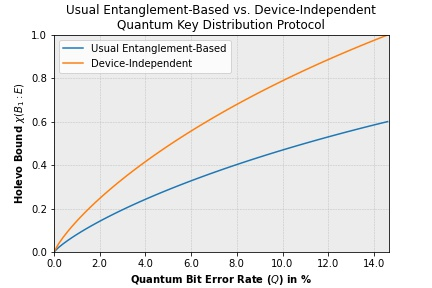
\includegraphics[width=\linewidth]{figures/presentation/jpg/holevo-bounds-quantum-bit-error-rate-plot.jpg}
                    \vspace{-4ex}
                \caption{\color{blue}{Figure 3: }\color{black}{Holevo bounds with respect to QBER $Q$}}
                \end{figure}
            \end{minipage}%
            \begin{minipage}{0.5\textwidth}
                \centering
                \vspace{0.5ex}
                \scriptsize $\sbullet$\, \textbf{For Devetak-Winter key rates:}\\
                \vspace{0.25ex}
                \tiny
                - Lower Devetak-Winter key rates for the DI-QKD protocol\\
                - The noise introduced by the eavesdropper will have greater impact on the DI-QKD protocol, reducing more the key rate\\
                - For a QBER $Q$ around $7\%$, no extractable secure raw key\\ will be possible in the DI-QKD protocol
                \vspace{-1.2ex}
                \begin{figure}
                    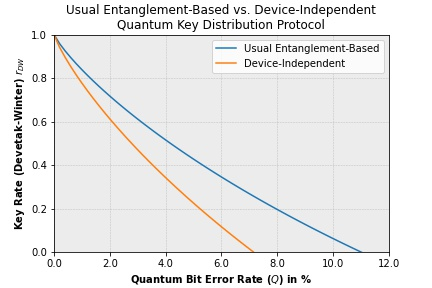
\includegraphics[width=\linewidth]{figures/presentation/jpg/key-rates-bounds-quantum-bit-error-rate-plot.jpg}
                    \vspace{-4ex}
                    \caption{\color{blue}{Figure 4: }\color{black}{Devetak-Winter key rates with respect to QBER $Q$}}
                \end{figure}
            \end{minipage}
            
		\end{frame}

		\begin{frame}
			\frametitle{\Large Possible loopholes for a DI‑QKD protocol}

            \vspace{3.5ex}
            \begin{itemize}
                \item \textbf{What is a loophole in Bell experiments?}
                \begin{itemize}
                    \item Flaw/gap in the experiment that may allow the results to:
                    \begin{itemize}
                        \item Be explained by local-hidden variables theory
                        \item Be falsely interpreted as violating Bell's Inequality due to imperfections or limitation in the design of the experiment
                    \end{itemize}
                \end{itemize}
                \item \textbf{There are two main loopholes in Bell experiments:}
                \begin{itemize}
                    \item \textbf{Locality loophole}
                    \begin{itemize}
                        \small
                        \item The quantum measurement devices can:\\
                        \footnotesize
                        - Be close to each other and/or delay their actions\\
                        - Communicate between themselves and influence the outcomes
                    \end{itemize}
                    \item \textbf{Detection loophole}
                    \begin{itemize}
                        \small
                        \item The quantum measurement devices can:\\
                        \footnotesize
                        - Fail to detect and measure all the incoming particles\\
                        - Not receive the incoming particles due to transmission losses
                    \end{itemize}
                    \vspace{1ex}
                    \item \textbf{Local models explain and determine these loopholes!}
                \end{itemize}
            \end{itemize}
		\end{frame}

		\begin{frame}
			\frametitle{\Large Possible loopholes for a DI‑QKD protocol}

            \vspace{3.5ex}
            \begin{itemize}
                \item \textbf{What is a loophole-free Bell experiment?}
                \begin{itemize}
                    \item A Bell experiment requiring:
                    \begin{enumerate}
                        \item A party cannot know any information about the other party's input before producing its own output
                        \item Measurement devices with high detection efficiencies\\
                        \footnotesize
                        - Ex.: A detection efficiency ${\eta}_{D} > 82.8\%$, for the CHSH Inequality
                    \end{enumerate}
                \end{itemize}
                \vspace{1ex}
                \item \textbf{Loopholes in the perspective of a DI-QKD protocol}
                \begin{itemize}
                    \item \textbf{How to circumvent the locality loophole?}
                    \begin{itemize}
                        \small
                        \item Considerable spatial separation between the parties\\
                        \footnotesize
                        - No sub-luminal signals travel between their quantum devices
                        \small
                        \item Proper and secure isolation of the parties' locations\\
                        \footnotesize
                        - No unwanted information can leak to the outside
                    \end{itemize}
                \end{itemize}
            \end{itemize}
		\end{frame}

		\begin{frame}
			\frametitle{\Large Possible loopholes for a DI‑QKD protocol}

            \vspace{3.5ex}
            \begin{itemize}
                \item \textbf{Loopholes in the perspective of a DI-QKD protocol}
                \begin{itemize}
                    \item \textbf{How to circumvent the detection loophole?}
                    \begin{itemize}
                        \small
                        \item (Possible) Post-selection on the measurement data\\
                        \footnotesize
                        - Discard no-detection events and keep only the events on which\\\hspace{0.5em}both quantum measurement devices produce an outcome
                        \vspace{0.75ex}
                        \small
                        \item Fair sampling assumption\\
                        \footnotesize
                        - The sample of detected particles is a fair, random\\\hspace{0.5em}and unbiased sample of the set of all particles\\
                        - No correlations between the quantum state of\\\hspace{0.5em}the particles and their detection probability\\
                        \vspace{1.5ex}
                        - Clearly unjustified for DI-QKD protocols, where we assume that\\\hspace{0.5em}the quantum devices can be provided by an untrusted party\\
                        \vspace{1.5ex}
                        - \textbf{This loophole still needs to be closed for DI-QKD protocols!}
                    \end{itemize}
                \end{itemize}
            \end{itemize}
		\end{frame}

		\begin{frame}
			\frametitle{\Large Possible loopholes for a DI‑QKD protocol}

            \vspace{3.5ex}
            \begin{itemize}
                \item \textbf{Handling detection loophole for a DI-QKD protocol}
                \begin{itemize}
                    \item \textbf{Addressing no-detection events for the security proof:}
                    \begin{itemize}
                        \small
                        \item We need to consider all the measurement outcomes\\
                        \footnotesize
                        - Detection ``$\pm1$'' and no-detection outcomes ``$\bot$''
                        \small
                        \item A possible strategy is to consider only two of them\\
                        \footnotesize
                        - Replace all no-detection outcomes ``$\bot$'' by outcome ``$-1$''
                    \end{itemize}
                    \vspace{1ex}
                    \item \textbf{How to overcome the detection loophole?}
                    \begin{itemize}
                        \small
                        \item \textbf{For quantum transmission losses:}\\
                        \footnotesize
                        - Use heralded quantum memories (with quantum repeaters)
                        \small
                        \item \textbf{For detector losses:}\\
                        \footnotesize
                        - Perform tomography tests only on the quantum detectors\\
                        - Use trusted quantum detectors or trusted calibration devices
                    \end{itemize}
                    \vspace{1ex}
                    \item For a detector efficiency ${\eta}_{D}$:
                    \begin{itemize}
                        \small
                        \item The CHSH polynomial's correlations satisfy now:\\
                        \footnotesize
                        $\sbullet$\, $Q = {\eta}_{D} (1 - {\eta}_{D})$
                        \hspace{2.5ex}
                        $\sbullet$\, $S = 2 \sqrt{2} {{\eta}_{D}}^{2} + 2 {(1 - {\eta}_{D})}^{2}$
                    \end{itemize}
                \end{itemize}
            \end{itemize}
		\end{frame}

		\begin{frame}
			\frametitle{\Large Possible loopholes for a DI‑QKD protocol}

            \vspace{3.5ex}
            \begin{itemize}
                \item Reformulating both the Holevo bound $\chi({B}_{1}:E)$ and\\ key rate ${r}_{DW}$, taking into account a detector efficiency ${\eta}_{D}$:
                \begin{itemize}
                    \item \textbf{For DI-QKD protocol:}
                    \begin{itemize}
                        \item $\chi({B}_{1}:E) = h\left( \frac{1 + \sqrt{{(\frac{S}{2})}^{2} - 1}}{2} \right) = $\\
                        \vspace{0.5ex}
                        \hspace{8ex}
                        $ = h\left( \frac{1 + \sqrt{{\left(\frac{ 2 \sqrt{2} {{\eta}_{D}}^{2} + 2 {(1 - {\eta}_{D})}^{2} }{2}\right)}^{2} - 1}}{2} \right)$
                        \item $r \geq {r}_{DW} = 1 - h(Q) - h\left( \frac{1 + \sqrt{{(\frac{S}{2})}^{2} - 1}}{2} \right) = $\\
                        \vspace{0.25ex}
                        \hspace{6.8ex}$= 1 - h({\eta}_{D} (1 - {\eta}_{D})) - h\left( \frac{1 + \sqrt{{\left(\frac{ 2 \sqrt{2} {{\eta}_{D}}^{2} + 2 {(1 - {\eta}_{D})}^{2} }{2}\right)}^{2} - 1}}{2} \right)$\\
                    \end{itemize}
                \end{itemize}
            \end{itemize}
		\end{frame}

		\begin{frame}
			\frametitle{\Large Possible loopholes for a DI‑QKD protocol}

            \vspace{3.5ex}
            \begin{itemize}
                \item Reformulating both the Holevo bound $\chi({B}_{1}:E)$ and\\ key rate ${r}_{DW}$, taking into account a detector efficiency ${\eta}_{D}$:
                \begin{itemize}
                    \item \textbf{For (usual) Entanglement-based QKD protocol:}
                    \begin{itemize}
                        \item $\chi({B}_{1}:E) = h\left( Q + \frac{S}{2 \sqrt{2}} \right) = $\\
                        \vspace{0.5ex}
                        \hspace{8ex}
                        $ = h\left( {\eta}_{D} (1 - {\eta}_{D}) + \frac{2 \sqrt{2} {{\eta}_{D}}^{2} + 2 {(1 - {\eta}_{D})}^{2}}{2 \sqrt{2}} \right)$
                        \item $r \geq {r}_{DW} = 1 - h(Q) - h\left( Q + \frac{S}{2 \sqrt{2}} \right) = $\\
                        \vspace{0.25ex}
                        \hspace{6.8ex}$= 1 - h({\eta}_{D} (1 - {\eta}_{D}))\, - $\\
                        \vspace{0.25ex}
                        \hspace{10ex}
                        $ -\, h\left( {\eta}_{D} (1 - {\eta}_{D}) + \frac{2 \sqrt{2} {{\eta}_{D}}^{2} + 2 {(1 - {\eta}_{D})}^{2}}{2 \sqrt{2}} \right)$\\
                    \end{itemize}
                \end{itemize}
            \end{itemize}
		\end{frame}

		\begin{frame}
			\frametitle{\large How to prove the security of a DI‑QKD protocol?}

            \vspace{4ex}
            \begin{itemize}
                \item How detector efficiencies ${\eta}_{D}$ impact the\\ (usual) Entanglement-based QKD and DI-QKD protocols?
            \end{itemize}
            
            \begin{minipage}{0.5\textwidth}
                \centering
                \vspace{0.5ex}
                \scriptsize
                $\sbullet$\, \textbf{For Holevo bounds:}\\
                \vspace{0.25ex}
                \tiny
                - Greater Holevo bounds for the DI-QKD protocol\\
                - We can detect the presence of an eavesdropper easier for\\ the DI-QKD protocol, but requiring higher detector efficiencies
                - For a detector efficiency ${\eta}_{D} = 83\%$, the eavesdropper has\\ all the information about the raw key in the DI-QKD protocol
                \vspace{-1.2ex}
                \begin{figure}
                    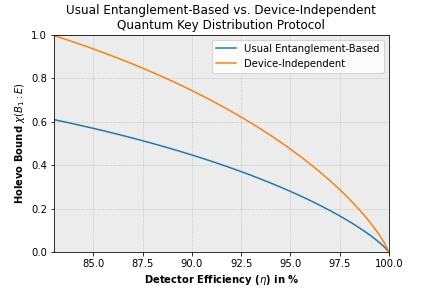
\includegraphics[width=\linewidth]{figures/presentation/jpg/holevo-bounds-detector-efficiency-plot.jpg}
                    \vspace{-4ex}
                \caption{\color{blue}{Figure 5: }\color{black}{Holevo bounds for a detector efficiency ${\eta}_{D}$}}
                \end{figure}
            \end{minipage}%
            \begin{minipage}{0.5\textwidth}
                \centering
                \vspace{0.5ex}
                \scriptsize $\sbullet$\, \textbf{For Devetak-Winter key rates:}\\
                \vspace{0.25ex}
                \tiny
                - Lower Devetak-Winter key rates for the DI-QKD protocol\\
                - The detector inefficiency will have greater impact\\ on the DI-QKD protocol, reducing more the key rate\\
                - For a detector efficiency ${\eta}_{D} = 92.4\%$, no extractable\\ secure raw key will be possible in the DI-QKD protocol
                \vspace{-1.2ex}
                \begin{figure}
                    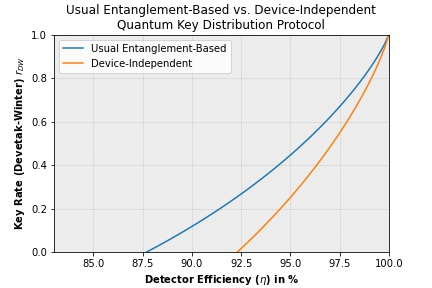
\includegraphics[width=\linewidth]{figures/presentation/jpg/key-rates-bounds-detector-efficiency-plot.jpg}
                    \vspace{-4ex}
                    \caption{\color{blue}{Figure 6: }\color{black}{Devetak-Winter key rates for a detector efficiency ${\eta}_{D}$}}
                \end{figure}
            \end{minipage}
            
		\end{frame}

    \section{Conclusion}

		\begin{frame}
			\frametitle{\Large Some possible directions and open questions}

            \vspace{3.5ex}
            \begin{itemize}
                \item \textbf{Possible directions:}
                \begin{itemize}
                    \item Consider other quantum cryptographic protocols:
                    \begin{itemize}
                        \item Based on different Bell inequalities
                        \item Even under the assumption of collective attacks 
                    \end{itemize}
                    \item Consider situations in which the eavesdropper may:
                    \begin{itemize}
                        \item Have partial information about measurement settings
                    \end{itemize}
                \end{itemize}
                \item \textbf{Open questions:}
                \begin{itemize}
                    \item \textbf{How is the security of the DI-QKD protocol modified\\ for two-way Information Reconciliation techniques?}
                    \begin{itemize}
                        \item Is a Bell inequality violation sufficient for security?
                    \end{itemize}
                    \item \textbf{Is de Finetti theorem extendable to the DI scenario?}
                    \begin{itemize}
                        \item Does the security against collective attacks implies security against the most general type of attacks?
                    \end{itemize}
                \end{itemize}
            \end{itemize}
            
		\end{frame}

    \section{Thanks for your attention!}

\end{document}